% !TEX root = ./multilinear.tex

\section{Proposed parallel algorithm: abstract description using a DAG representation}
\label{sec:proposed}
We first describe a parallel algorithm for the $k$-MLD problem, using a DAG representation
for a multivariate polynomial $P(\cdot)$.  
Both problems \ref{prob:trees} and \ref{prob:macs} can be reduced to instances
of the $k$-MLD problem, as we will discuss later in Section \ref{sec:applications};
this will automatically lead to corresponding parallel algorithms for both these problems.
We note that the DAG representation used in this section
is only for the purpose of explaining the parallel algorithm for both these problems; we do not
solve the two problems by explicitly constructing DAGs. The specific algorithms
for the two problems in Section \ref{sec:application} involve \emph{implicit construction} of DAGs.

%\subsection{Overview of the Algorithm \parmaxwt{}}
%We assume a DAG $D$, which represents an instance of $k$-MLD, with levels $\mathcal{L} = \{L_1,\ldots,L_{|\mathcal{L}|}\}$. The algorithm involves
%evaluating the DAG in $2^k$ iterations, which are partitioned into ``phases'' of $N_2$ iterations each;
%therefore, a total of $2^k/N_2$ phases have to be run.
%For $t\geq 1$, the $t$th phase involves the iterations $tN_2, tN_2+1,\ldots, (t+1)N_2-1$.  
%The idea is that a phase will be run simultaneously using $N_1$
%processors. Let $N$ denote the total number of processors available. Therefore, $N/N_1$
%phases can be done in parallel, which require $\frac{2^k/N_2}{N/N_1}$
%iterations of the while loop.

\subsection{Overview of the Algorithm \parmaxwt{}}
Let DAG $D(V,E)$ be the equivalent representation to a multivariate polynomial $P(\cdot)$.
Let $N$ denote the total number of
processors. Quantities $N_1$ and $N_2$ are parameters for controlling the parallelism
in different parts.  
We assume $2^k/N_2$ and $N/N_1$ are integers, in order to avoid cluttering the
notation using ceiling and floor of these quantities, respectively.
The algorithm involves evaluating the
DAG for a constant number of rounds; each round consists of
$2^k$ iterations, which are partitioned into ``phases'' of $N_2$ iterations each,
so that a total of $2^k/N_2$ phases have to be run. These are run in $2^k/(N_2N/N_1)$ ``batches'',
where each batch involves running $N/N_1$ phases. A phase involves a call to the subroutine \parcircuit{}.
See Figure \ref{fig:parallel} for an illustration of this structure.

We assume $D$ has levels $\mathcal{L} = \{L_1,\ldots,L_{|\mathcal{L}|}\}$. 
The DAG is partitioned into $N_1$ parts, denoted by
$\mathcal{P}=\{D^1, \ldots, D^{N_1}\}$; desirable properties of
the partition will be discussed later.
%$\mathcal{P}=\{G^1= (V^1, E^1), \ldots, G^{N_1}=(V^{N_1}, E^{N_1})\}$.
For each level $L_s\in\mathcal{L}$, let $L_s^j$ denote the corresponding level
in partition $j$; $\mathcal{L}^j$ denotes the set of all levels in that partition.
For level $L_s\in\mathcal{L}$, let $\maxload{}_s = \max_j |L_s^j|$ be the maximum
``load'' on partition $j$ from that level. Further, for $s<|\mathcal{L}|$, let
$\maxdeg{}_s = \max_{j\neq j'} |\{(u, v)\in L_s\times L_{s+1}: u\in L_s^j, v\in L_{s+1}^{j'}\}|$
denote the maximum number of edges from any $L_s^j$ to $L_{s+1}^{j'}$.
We will analyze the performance of our algorithm in terms of $\maxload{}_s$ and $\maxdeg{}_s$.

\begin{figure}[h]
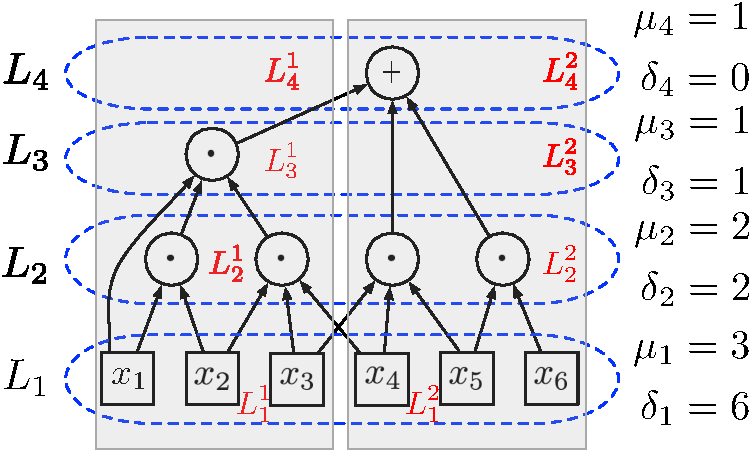
\includegraphics[width=0.4\textwidth]{img/dag4.pdf}
\caption{
\small
Illustration of the level sets and associated quantities for the DAG in
Figure \ref{fig:dag}, corresponding to a partition into two parts. 
%\vspace{-0.2in}
}
\label{fig:dag4}
\end{figure}

\noindent
\textbf{High level overview.}
We describe the main intuition of the steps of Algorithm \parmaxwt{} below.
\begin{enumerate}
\item
The algorithm starts with the partitioning $\mathcal{P}$ of the graph $D$.
%We discuss its complexity and implementation in Section \ref{sec:partition}.
\item
The algorithm runs $\log{1/\epsilon}\log{5/4}$ rounds, each of which involves $2^k$ iterations.
Here $\epsilon\in(0, 1)$ is a parameter, which governs the success probability.
Each such round with $2^k$ iterations is partitioned into
$2^k/N_2$ phases in the while loop in lines 10-15 of \maxwt{}, which
are completely independent of other phases.
\item
In the $t$th phase, Algorithm \parcircuit{} uses a vector of size $N_2$ to store
$\val(i) = \langle \val(i, tN_2),\ldots, \val(i, (t+1)N_2-1)\rangle$ for each node $i$; these
will be computed simultaneously using a dynamic program.
\item
In the $t$th phase, for each node $i$, we use the vector
$\val(j)$ for each predecessor $j$ of $i$ to compute $\val(i)$.
If $j$ is in the same partition $p'$, then $\val(j)$ is available on that processor.
For every predecessor $j$ in a different partition, 
$j$ has to send a message with $\val(j)$, introducing a communication overhead.
\item
We use $\rootsum^{\ell}_t = \val(\text{root}, tN_2) + \ldots \val(\text{root}, (t+1)N_2-1)$ 
to denote the sum of the values of the root node within the phase, for round $\ell$. These are summed up
over all the phases within round $\ell$ to compute the total, denoted by $M_{\ell}$.
\end{enumerate}

\begin{figure}[h]
\centering
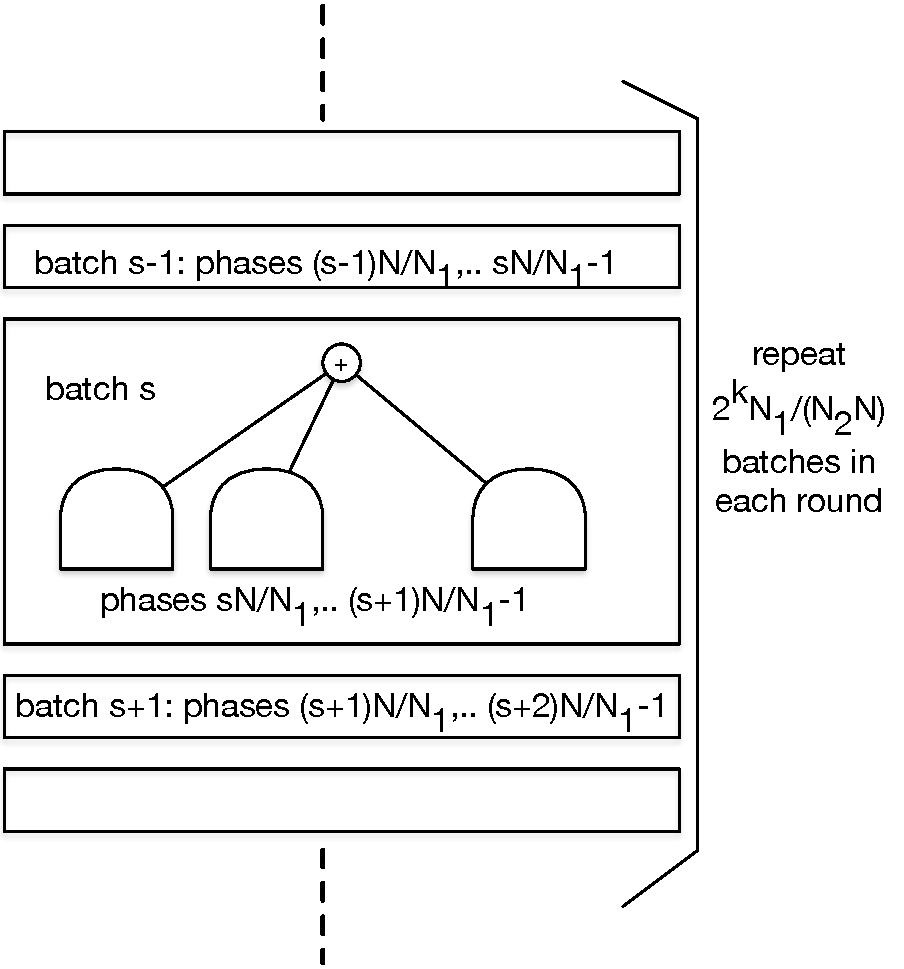
\includegraphics[width=0.3\textwidth]{img/parallel.pdf}
\caption{
\small
Schematic structure of \parmaxwt{}: we run $(\log{1/\epsilon})/(\log{5/4})$ rounds.
Each round is partitioned into $2^kN_1/(N_2N)$ batches, and each batch involves
$N/N_1$ phases being run simultaneously. Each phase involves a evaluation of the
polynomial/DAG on $N_2$ iterations in algorithm \parcircuit{}, which are then summed up.
}
\label{fig:parallel}
\end{figure}

\begin{algorithm}{}
\small
\caption{\parmaxwt{}$(D, k, \mathcal{L}, \epsilon, N_1, N_2)$.}
\label{alg:parallel-kMLD} 
\begin{algorithmic}[1]
\STATE \textbf{Input}: Circuit $D$, parameter $k$, node levels $\mathcal{L}$,
confidence parameter $\epsilon\in (0, 1)$, parameters $N_1$ and $N_2$, which guide the parallelism.
\STATE\textbf{Output}: ``True" if circuit evaluation is non-zero. ``False" otherwise.

\STATE Let $v_i \in \mathbb{Z}_2^k$ be a random vector for each node $i$
\STATE Let $M = \bar 0$ be the polynomial
\STATE Let $N_1$ denote the number of processors used for each iteration.
%Let $\mathcal{P}=\{G^1= (V^1, E^1), \ldots, G^{N_1}=(V^{N_1}, E^{N_1})\}$ denote the corresponding
Let $\mathcal{P}=\{D^1, \ldots, D^{N_1}\}$ denote the corresponding
partition of the graph into $N_1$ parts.
\STATE \textbf{for} $\ell=1$ to $(\log{1/\epsilon})/(\log{5/4})$ 
\STATE \quad $M^{\ell}=0$
\STATE \quad \textbf{while} $s \leq \frac{2^k/N_2}{N/N_1}$ \textbf{do}
\STATE \quad \quad \textbf{for} $t =s N/N_1$ to $(s+ 1)N/N_1$ \textbf{do in parallel}
\STATE \quad \qquad  $\rootsum^{\ell}_{t} = \parcircuit(D, k, \mathcal{L}, \mathbf{v}, t, N_2, N_1, \mathcal{P})$
\STATE \quad \quad \textsc{MpiBarrier}
\STATE \quad \quad $M^{\ell} = M^{\ell} + \sum_{t=s N/N_1}^{(s+1)N/N_1} \rootsum^{\ell}_{t} \mod 2^{k+1}$ using \textsc{MpiReduce}
\STATE \textbf{if} $M^{\ell}\neq 0$ for some $\ell$
\STATE \quad \textbf{return} \textbf{True}
\STATE \textbf{else} 
\STATE \quad \textbf{return} \textbf{False}
\end{algorithmic}
\end{algorithm}

\begin{algorithm}{}
\small
\caption{\parcircuit{$(D, k, \mathcal{L}, \mathbf{v}, t, N_2, N_1, \mathcal{P})$}}
\label{alg:parEvaluate} 
\begin{algorithmic}[1]
%\STATE \textbf{Procedure} \parcircuit{$(G(V, E), k, \mathcal{L}, \mathbf{v}, t, p)$}
\STATE \textbf{Input:} Circuit $D$, parameter $k$, node levels $\mathcal{L}$, 
random assignment $\mathbf{v}$, phase number $t$, number of iterations within phase $N_2$,
number of partitions $N_1$, and partitioning $\mathcal{P}$
\STATE
\STATE \textbf{for} processor $p'$ \textbf{do in parallel}
\STATE \quad \textbf{Initialize circuit inputs}
\STATE \quad \textbf{for} node $i \in L^{p'}_{1}$ and iteration $q$ in $tN_2,\ldots,(t+1)N_2-1$ \textbf{do}
\STATE \qquad $ \val(i, q) = 1 + (-1)^{v_i^T \cdot q_{\text{bin}}}$

\STATE \quad \textbf{Evaluate the circuit by levels}
\STATE \quad \textbf{for} $s=2$ to $|\mathcal{L}^{p'}|$ \textbf{do}
\STATE \qquad \textbf{for} $i \in L_s^{p'}$ \textbf{do}
\STATE \qquad \quad \textbf{if} $\op(i) = +$ \textbf{then}
\STATE \qquad \qquad \textbf{for} all $q$ set $\val(i,q) = \bar 0$
\STATE \qquad \qquad \textbf{for} $j \in \pred(i)\cap V^{p'}$  \textbf{do}
\STATE \qquad \qquad \quad \textbf{for} all $q$: $\val(i, q) = \val(i, q) + \val(j, q)$
\STATE \qquad \qquad \textbf{for} each incoming message $\langle j, \val(j)\rangle$ \textbf{do}
\STATE \qquad \qquad \quad \textbf{for} all $q$: $\val(i, q) = \val(i, q) + \val(j, q)$
\STATE \qquad \quad \textbf{else} 
\STATE \qquad \qquad \textbf{for} all $q$: $\val(i, q) = \bar 1$
\STATE \qquad \qquad \textbf{for} $j \in \pred(i)\cap V^{p'}$ \textbf{do}
\STATE \qquad \qquad \quad \textbf{for} all $q$: $\val(i, q) = \val(i, q) \cdot \val(j, q)$
\STATE \qquad \qquad \textbf{for} each incoming message $\langle j, \val(j)\rangle$ \textbf{do}
\STATE \qquad \qquad \quad \textbf{for} all $q$: $\val(i, q) = \val(i, q) \cdot \val(j, q)$
\STATE \qquad \quad  \textbf{Send result to successors in other processors}
\STATE \qquad \quad \textbf{for} $j \in \succ(i) \setminus V^{p'}$ \textbf{do}
\STATE \qquad \qquad \textbf{Send} $\langle i, \val(i)\rangle$
\STATE \textsc{MpiBarrier}
\STATE \textbf{return} $\sum_q \val($root$, q)$
\end{algorithmic}
\end{algorithm}

Recall the definitions of $\maxload{}_s$ and $\maxdeg{}_s$ corresponding to the partitioning
$\mathcal{P}$ and corresponding level decomposition $\mathcal{L}^j, j=1,\ldots,p$.
Further, let $c_1$ and $c_2$ denote the time for unit computation at any node in $D$
and the unit communication along any edge, respectively, in the Algorithm \parcircuit{}.
The time and communication complexity of algorithm \parmaxwt{} is summarized below
in terms of these parameters. 

\begin{theorem}
\label{thm:parmaxwt}
For any $\epsilon\in(0, 1)$,
Algorithm \parmaxwt{} solves the \textsc{$k$-MLD} problem for an
instance $P(x_1,\ldots,x_n)$ with probability at least $1-\epsilon$. The total time for
computation and communication are $O\left(c_1\frac{2^kN_1}{N}\sum_s \maxload{}_s\log{1/\epsilon}\right)$ 
and $O\left(c_2\frac{2^kN_1}{N N_2}\sum_s \maxdeg{}_s\log{1/\epsilon}\right)$, respectively.
\end{theorem}
\begin{proof} (Sketch)
First, we argue the correctness. 
The DAG is an equivalent representation of the polynomial $P(\cdot)$. 
The call to \parcircuit{} evaluates the DAG bottom up in parallel for all iterations in the
$t$th phase, namely iterations $tN_2,\ldots,(t+1)N_2-1$. The vector
$\val(\text{root})=\langle \val(\text{root}, tN_2),  \ldots ,\val(\text{root}, (t+1)N_2-1)\rangle$
is the evaluation of the root of the DAG for each iteration in this phase.
Each call to \parcircuit{} in Algorithm \parmaxwt{}
returns the sum of these values at the root for phase $t$.
Each round of Algorithm \parmaxwt{}, corresponding to the value of
$\ell$ in the outer for loop in lines 6--12, goes over all phases, and
calls \parcircuit{}. Therefore, within round $\ell$, $M^{\ell}$ denotes the
sum of the DAG/polynomial evaluation over all the $2^k$ iterations within that round.
If $P(\cdot)$ has a multilinear term,
from \cite{koutis:icalp08,williams2009finding}, $M^{\ell}\neq 0 \text{ mod }2^{k+1}$ with
probability at least $1/5$. This implies that 
$\Pr[M^{\ell} = 0,\ \forall \ell] = (\frac{4}{5})^{(\log{1/\epsilon})/(\log{5/4})}\leq\epsilon$,
so that with probability at least $1-\epsilon$, \parmaxwt{} returns true.  On the other hand,
if $P(\cdot)$ has no multilinear term, then with probability $1$, $M^{\ell}=0$ for all $\ell$.
Therefore, \parmaxwt{} correctly solves the \textsc{$k$-MLD} problem with probability
at least $1-\epsilon$.

Next, we consider the computation and communication time complexity. 
The algorithm \parcircuit{} computes the DAG level by level within each iteration.
Therefore, the computation time for level $s\leq |\mathcal{L}|$ in a phase $t$ is 
$O(c_1\max_j |L_s^j| N_2) = O(c_1\maxload{}_sN_2)$, which is the maximum time for any processor
for this level. Therefore, the total compute time over all the rounds is
$O(\frac{2^k/N_2}{N/N_1} c_1\maxload{}_sN_2)$, which corresponds to the bound in the theorem.
After any level $s$ is computed, the results have to be sent on all edges in the set 
$\{(u, v)\in L_s\times L_{s+1}: u\in L_s^j, v\in L_{s+1}^{j'}\}$, for every pair of
processors $j, j'$. Therefore, the maximum number of messages after level $s$ is
$\maxdeg{}_s = \max_{j\neq j'} |\{(u, v)\in L_s\times L_{s+1}: u\in L_s^j, v\in L_{s+1}^{j'}\}|$.
Therefore, the total number of messages, over all the rounds, is
$O(\frac{2^k/N_2}{N/N_1} \sum_s \maxdeg{}_s) = O(\frac{2^kN_1}{N N_2}\sum_s \maxdeg{}_s)$.
\end{proof}

%%\subsection{Partition and Load Balancing}
%%\label{sec:partition}
%%
%%From Theorem \ref{thm:parmaxwt}, the performance of Algorithm \parmaxwt{} depends crucially
%%on the partitioning. Specifically, the partition should be ``vertical'', i.e., one which achieves
%%load balance across each level and also minimizes the edge cut, which is formalized by
%%\[
%%\text{cost}(\mathcal{P}) = \sum_s (c_1\maxload{}_s + c_2\maxdeg{}_s)
%%\]
%%
%%However, finding a partitioning $\mathcal{P}$ that minimizes the above objective
%%$\text{cost}(\mathcal{P})$ is NP-hard, in general, as summarized below. The proof
%%is omitted for brevity.
%%
%%\begin{lemma}
%%\label{lemma:partition}
%%Given a DAG $G=(V, E)$ and per-unit computation and communication costs $c_1$ and $c_2$,
%%respectively, finding a partitioning $\mathcal{P}$ with the minimum cost is NP-hard, in general.
%%\end{lemma}
%%
%%In light of Lemma \ref{lemma:partition}, we consider two heuristics: finding balanced
%%partitions in each level, and combining them, as well as METIS \cite{karypis:sijsc99}.

%We partition the circuit ``vertically"; that is, each processor gets a subset of nodes for each level in $\mathcal{L}$. Let $f(i)$ be the cost of evaluating node $v$. Then, we want to find a partition, such that
%$$
%\sum_{v \in V^p} f(i) \approx \frac{1}{p}\sum_{i \in V} f(i).
%$$

%\subsection{Analysis of Algorithm \parmaxwt{}}
%\subsubsection{Time Complexity}
%The \textbf{while} loop in lines 8--13 of \parmaxwt{} runs for at most $\frac{2^k}{P / p}$ iterations. For each iteration, each partition does work in the order $O(\frac{1}{p}\sum_{i \in V} f(i))$, so the total running time is $O(\frac{1}{p}(2^k f(V)))$.
%\subsubsection{Number of Messages}
%We assume that we have $P$ processors available and that $G$ does not fit in the memory of a single computing node. We have to use $p \leq P$ processors to store the graph in memory. We propose an MPI algorithm with roughly the following steps:

%\begin{enumerate}
%\item \parmaxwt{} Algorithm \ref{alg:parallel-kMLD}
%\item Determine $p$, the number of processors needed to store the graph.
%\item We have to run the loop from line 9 of \maxwt{}. Each of the $2^k$ iteration is independent of the others, so we can run $\lfloor{P/p}\rfloor$ iterations in parallel.
%\item \parcircuit{} Algorithm \ref{alg:parEvaluate}
%\item For each iteration $t$, we first partition the circuit into $p$ parts, and we evaluate these parts in parallel.
%\item For each partition $p'$, we evaluate the circuit by levels, as in \maxwt{}. 
%\item For each node $i$ that we evaluate, we compute $m(i)$ using the $m(j)$ value for each predecessor $j$. if a predecessor $j$ is in the same partition $p'$, then, we can simply read $m(j)$, as in the sequential algorithm. For every predecessor $j$ in a different partition, $j$ has to send a message with $m(j)$, introducing a communication overhead.
%\item We aggregate the value at root$(G)$ over all $2^{k}$ iterations to get the final solution.
%\end{enumerate}

%\noindent
%\textbf{Algorithm \ref{alg:parallel-kMLD}}: \parmaxwt{}\\
%1. Determine $p$, the number of processors needed to store the graph.\\
%2. We have to run the loop from line 9 of \maxwt{}. Each of the $2^k$ iteration is independent of the others, so we can run $\lfloor{P/p}\rfloor$ iterations in parallel.\\
%\textbf{Algorithm \ref{alg:parEvaluate}}: \parcircuit{} \\
%3. For each iteration $t$, we first partition the circuit into $p$ parts, and we evaluate these parts in parallel.\\
%4. For each partition $p'$, we evaluate the circuit by levels, as in \maxwt{}. \\
%5. For each node $i$ that we evaluate, we compute $m(i)$ using the $m(j)$ value for each predecessor $j$. If a predecessor $j$ is in the same partition $p'$, then, we can simply read $m(j)$, as in the sequential algorithm. For every predecessor $j$ in a different partition, $j$ has to send a message with $m(j)$, introducing a communication overhead.\\
%6. We aggregate the value at root$(G)$ over all $2^{k}$ iterations to get the final solution.
